\section{はじめに}
自宅サーバー,憧れますよね.そんな自宅サーバーをお手頃な価格で自作してしまいましょう.せっかくなのでモーターとタイヤをつけてしまいましょう.そうです,自走式WEBサーバーです.この章ではWiFiを扱うことのできるマイコン ESP-WROOM-02を用いた自走式WEBサーバーを作成します.(図 \ref{fig:webserver})
\footnote{本章に記載されたプログラム,回路図,その他工作物を参考にして製作した場合に生じた事故等について一切の責任を負いかねます.}
\subsection{ESP-WROOM-02とは}
ESP-WROOM-02は,上海の企業Espressif Systems のESP8266EXチップを搭載したWiFiモジュールです.いわゆる「技適」を取得しているため,日本国内で法的に安心して使えます.ardiono言語で開発できることに加え,おおよそ600円で購入できる手軽さが魅力です.
\footnote{ESP-WROOM-02の開発環境の構築方法については, ESP8266 Arduino Coreの公式ドキュメント(\url{https://arduino-esp8266.readthedocs.io/en/latest/})や,僕のブログ(\url{https://haibara-works.hatenablog.com})の『ESP-WROOM-02を導入する』を参照してください.(ページ数の都合から本章ではその説明は割愛します)}

\begin{figure}[htbp]
    \centering
    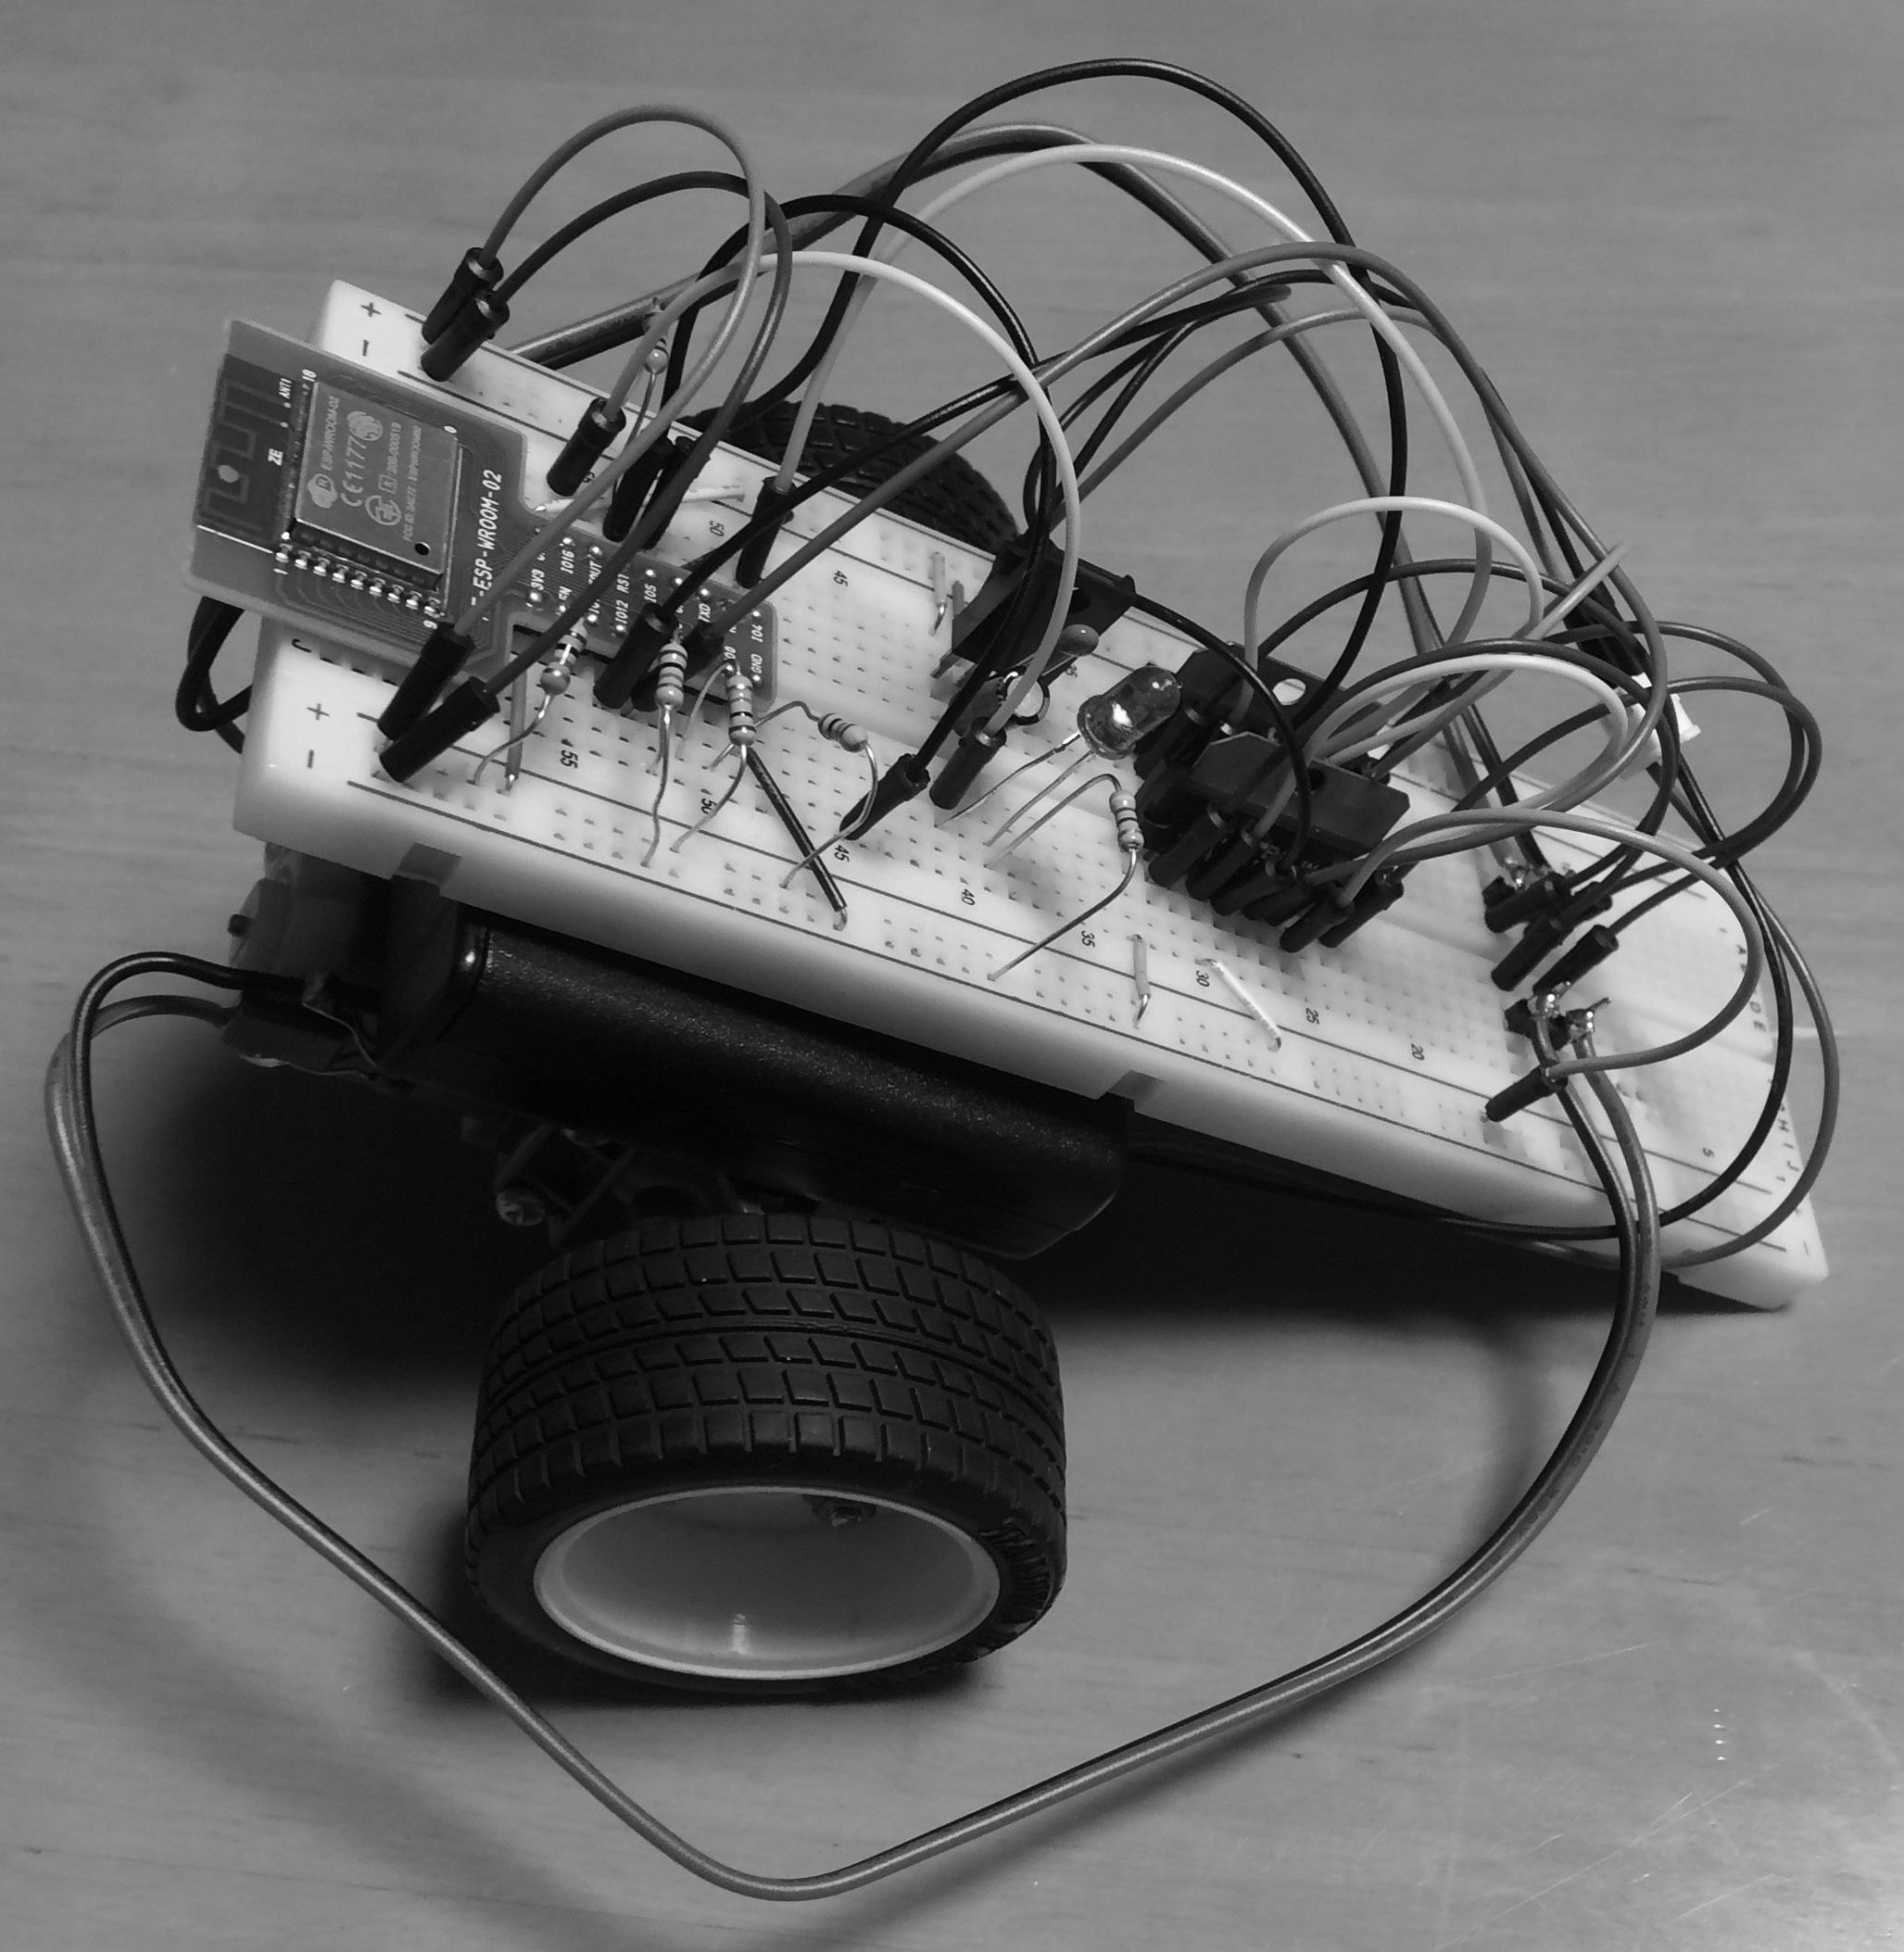
\includegraphics[width=50mm]{./assets/haibaraaaaaaaasset/webserver.jpg}
    \caption{自走式Webサーバーの実装例}
    \label{fig:webserver}
\end{figure}

\subsection{ハードウェアの準備}
表\ref{buhin}に今回作る自走式WEBサーバーに必要な部品を示します.
\begin{table}[htb]
\centering
\caption{使うもの}
\begin{tabular}{|l|l|} \hline
部品 & 用途 \\ \hline \hline
ESP-WROOM-02 & ESP本体  \\ \hline
FT-232RQ & USBシリアル変換モジュール  \\ \hline
抵抗(10 K$\Omega$) & プルアップ・プルダウン用  \\ \hline
抵抗(470 K$\Omega$) & LEDの保護抵抗 \\ \hline
LED & パイロットランプ  \\ \hline
TA48033S & 電源レギュレータ(3.3 V) \\ \hline
コンデンサ(0.33 $\mu$F) & 電源用パスコン  \\ \hline
コンデンサ(33 $\mu$F) & 電源用パスコン  \\ \hline
TA7291P & モータードライバ \\ \hline
ダブルギヤボックス(左右独立4速タイプ) & タミヤのギヤボックス  \\ \hline
ブレッドボード & テスト用 \\ \hline
ジャンパ線 & テスト用 \\ \hline
\end{tabular}
\label{buhin}
\end{table}

\section{ラジコンとしての動作}
\subsection{モータードライバの利用}
    モーターの制御にはモータードライバIC TA7291Pを使用します.このICはArduinoの入門記事などでよく登場する,とても扱いやすいICです.制御方法も簡単で,2つの入力端子をマイコンのGPOに接続し,2つの出力をモーターのそれぞれの端子に接続して使います.以下にTA7291Pの真理値表を示します.
\footnote{表中のZはハイインピーダンス(LともHとも定まらない状態)を表します}
\footnote{正転・逆転はモーターの端子とOUT1・OUT2との接続の仕方によっては逆になります.}

\begin{table}[H]
\centering
\caption{TA7291Pの動作}
\begin{tabular}{|l|l|l|l|l|} \hline
IN1 & IN2 & OUT1 & OUT2 & 用途 \\ \hline \hline
L & L & Z & Z & オープン \\ \hline
L & H & L & H & 正転 \\ \hline
H & L & H & L & 逆転 \\ \hline
H & H & L & L & ブレーキ \\ \hline
\end{tabular}
\label{buhin}
\end{table}

また,真理値表の正転・逆転の際のHをPWM出力にすれば,PWM波形のデューティ比に応じたスピードでモーターを制御することができます.
つまり,以下のコードがTA7291Pを用いたモーター制御の基本になります.
\begin{minted}[frame=lines,framesep=2mm,baselinestretch=1.2,fontsize=\footnotesize,linenos,breaklines]{c}
analogWrite(motorPin1, pwmValue);
digitalWrite(motorPin2, LOW);
\end{minted}
これを左右のモーターそれぞれに適応させ,前進・後進・右旋回・左旋回をさせます.

\subsection{Webからの操作}
Webページからモーターを制御するために,URLクエリ文字列を利用します.URLクエリ文字列とはURLに付帯する引数のようなもので,たとえば\url{192.168.4.10/?val=abc}というURLであれば"valという引数の値はabcである"と解釈されます.また\url{192.168.4.10/?val1=abc&val2=123}というように\&で結ぶことで複数の引数を付帯させることもできます.ESPでは\tt{ESP8266WebServer.h}\rm{}でURLクエリ文字列の取得に関するかいくつかの関数が定義されています.次の関数はそれらの使用例です.
\begin{minted}[frame=lines,framesep=2mm,baselinestretch=1.2,fontsize=\footnotesize,linenos,breaklines]{c}
/**  Show URI args */
void showUriArgs() {
  Serial.println("---URI args---");
  for (int i = 0; i < Server.args(); i++) { //Server.args(): クエリ文字列の引数の個数を取得
    Serial.printf("%s: %s \n", Server.argName(i).c_str(), Server.arg(i).c_str()); 
    //Server.argName(num): クエリ文字列のnum番目の引数名を取得
    //Server.arg(num); クエリ文字列のnum番目の引数の値を取得
  }
}
\end{minted}
ESPに\url{192.168.4.10/?val1=abc&val2=123}というURLへリクエストがあった際にこの関数が実行されると,シリアルコンソールには
\tt{

---URL args---

val1: abc

val2: 123

}\rm{}
と表示されるはずです.
また,\tt{Server.arg("val")}\rm{}というように\tt{Server.arg()}\rm{}にクエリ文字列の引数名を渡すと,その引数の値を取得できます.
今回のコードではWebサーバーの進行方向をmotorModeで,モーターの回転速度をmotorValでそれぞれ指定することにします.
ボタンとスライダーでこれら2つの値を指定する簡易的な操作画面をHTMLとjsで示しました.(図 \ref{fig:html})

\begin{figure}[htbp]
    \centering
    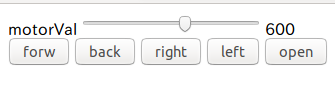
\includegraphics[width=50mm]{./assets/haibaraaaaaaaasset/motorCtr.png}
    \caption{自走式Webサーバーの操作画面}
    \label{fig:html}
\end{figure}

\begin{minted}[frame=lines,framesep=2mm,baselinestretch=1.2,fontsize=\footnotesize,linenos,breaklines]{c}
enum { M1_l = 4, M1_r = 5, M2_l = 12, M2_r = 13, Pilot = 16, //モーターを接続するピン及びパイロットランプを接続するピンの定義
       Stop, Open, Forw, Back, Right, Left }; //motorModeの値となる定数

typedef struct {
  int _mode; //Webサーバーの進行方向を格納
  int val; //モーターの回転速度を格納
} motor_T;
motor_T motor;

/**************************************************
  モーター制御に関する関数群
 **************************************************/
/**  左右2つのモーターに接続されるピンを初期化 */
void motorSetup(const int m1_l, const int m1_r, const int m2_l, const int m2_r) {
  pinMode(m1_l, OUTPUT);
  pinMode(m1_r, OUTPUT);
  pinMode(m2_l, OUTPUT);
  pinMode(m2_r, OUTPUT);

  digitalWrite(m1_l, LOW);
  digitalWrite(m1_r, LOW);
  digitalWrite(m2_l, LOW);
  digitalWrite(m2_r, LOW);

  analogWriteFreq(5);
}

/**  モーターをPWM制御する関数 */
void motorDrive(int16_t pwmVal, const int m_l, const int m_r) {
  pwmVal = constrain(pwmVal, -1024, 1024);

  if (pwmVal >= 0) {
    analogWrite(m_l, pwmVal);
    digitalWrite(m_r, LOW);
  } else {
    pwmVal = abs(pwmVal);

    digitalWrite(m_l, LOW);
    analogWrite(m_r, pwmVal);
  }
}

/**  stop */
void stopMotor() {
  digitalWrite(M1_l, LOW);
  digitalWrite(M1_r, LOW);
  digitalWrite(M2_l, LOW);
  digitalWrite(M2_r, LOW);
}

/**  前進 */
void goForward(int16_t velocity) {
  motorDrive(velocity, M1_l, M1_r);
  motorDrive(velocity, M2_l, M2_r);
}

/**  後進 */
void goBack(int16_t velocity) {
  motorDrive(-velocity, M1_l, M1_r);
  motorDrive(-velocity, M2_l, M2_r);
}

/**  右旋回 */
void turnRight(int16_t velocity) {
  motorDrive(velocity, M1_l, M1_r);
  motorDrive(-velocity, M2_l, M2_r);
}

/**  右旋回 */
void turnLeft(int16_t velocity) {
  motorDrive(-velocity, M1_l, M1_r);
  motorDrive(velocity, M2_l, M2_r);
}
\end{minted}

\section{WEBサーバーとしての動作}
最低限のWEBサーバーとして,クライアントがHTTP GETでページを取得できること,不揮発性メモリにファイルを保存できること,不揮発性メモリ内のファイルを作成・改変・削除できるようにすること,の3つの機能を実装しました.
\subsection{SPIFFSの利用}
ESPではSPIFFSというファイルシステムを使うことが出来ます.これはESPの不揮発性メモリの一部をストレージとして使えるようにするもので,プログラム中からC言語の\tt{fopen()}\rm{} と同じ要領でメモリにアクセス出来ます.この機能を用いてESPにファイルを保存します.
また,ArduinoIDEにSPIFFSプラグイン(\url{https://github.com/esp8266/arduino-esp8266fs-plugin})をインストールすると,ArduinoIDEからESPのSPIFFSにファイルをアップロードすることができます.
ESP8266 Arduino Coreの公式exampleの中にFSBrowserというスケッチが,まさにSPIFFSを用いたWebサーバーの実装になっています(\url{https://github.com/esp8266/Arduino/tree/master/libraries/ESP8266WebServer/examples/FSBrowser}).
このスケッチにある関数\tt{String formatBytes(size\_t bytes)}\rm{}・\tt{bool handleFileRead(String path)}\rm{}・\tt{void handleFileUpload()}\rm{}・\tt{void handleFileDelete()}\rm{}・\tt{void  handleFileCreate()}\rm{}・\tt{void  handleFileList()}\rm{}を利用します.
また,FSBrowser.inoと同じディレクトリの\tt{/data}\rm{}内にはいくつかのjsファイルやhtmlファイルが保存されています.その中にはSPIFFSに保存されているファイルの編集・改変・削除,新規ファイルのアップロードを行うことのできるWebGUIとして働くものや,現在のヒープメモリやGPIOの電位などをグラフで提供するものが含まれています.(図 \ref{fig:fsb})今回はこれらの\tt{/data}\rm{}内のファイルを使用して,SPIFFS管理のためのWebGUIとします.

\begin{figure}[htbp]
    \centering
    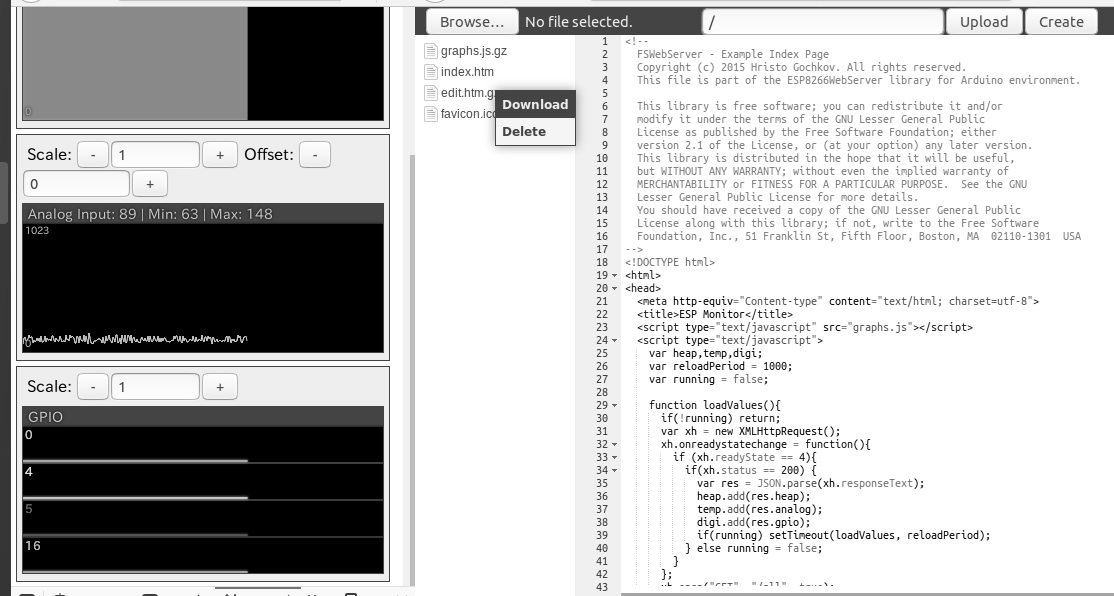
\includegraphics[width=50mm]{./assets/haibaraaaaaaaasset/FSBrowser.png}
    \caption{FSBrowserのWebGUI}
    \label{fig:fsb}
\end{figure}

\subsection{Webページの表示}
\tt{ESP8266WebSerber.h}\rm{}を用いて,クライアントからのHTTPリクエストを処理する際には,\tt{Server.on(path, handlerFunction);}\rm{}と記述することで,"\tt{path}\rm{}がリクエストされたら\tt{handlerFunction}\rm{}を実行する"ということができます.しかし,この方法では処理できる\tt{path}\rm{}の種類がコーディングの時点で固定されてしまいます.今回のようにSPIFFSを用いて,動的にファイルが変わり得る場合はどのように対処すればいいでしょうか.1つの方法は\tt{Server.on(path, handlerFunction)}\rm{}ではなく\tt{Server,onNotFound(handlerFunction)}\rm{}を用いることです.これはクライアントにリクエストされた\tt{path}\rm{}がどの\tt{Server.on}\rm{}でも指定されていない場合に,\tt{handlerFunction}\rm{}を呼び出すという関数で,その名の通り404 Not Foundを返すために使われます.しかし\tt{Server.on}\rm{}を記述しなければ任意の\tt{path}\rm{}がリクエストされたときに必ず\tt{handlerFunction}\rm{}が呼ばれます.この\tt{handlerFunction}\rm{}内で"リクエストされた\tt{path}\rm{}はSPIFFSに存在するか"を判断し,存在すればその\tt{path}\rm{}ごとの処理をし,存在しなければ404 Not Foundをクライアントに送信するという処理を行うことで,SPIFFS内の動的ファイルの変化に対応できます.

\begin{minted}[frame=lines,framesep=2mm,baselinestretch=1.2,fontsize=\footnotesize,linenos,breaklines]{c}
#include <ESP8266WiFi.h>
#include <WiFiClient.h>
#include <ESP8266mDNS.h>
#include <ESP8266WebServer.h>
#include <ESP8266HTTPUpdateServer.h>
#include <FS.h>
#include "config.h"

const char* host = "esp8266fs";
ESP8266WebServer Server(80);      //80番ポートを使用

/**************************************************
  WEBサーバーに関する関数群
 **************************************************/
/**  Show URI args */
void showUriArgs() {
  Serial.printf("\n---URI args---\n");
  for (int i = 0; i < Server.args(); i++) {
    Serial.printf("%s: %s \n", Server.argName(i).c_str(), Server.arg(i).c_str());
  }
}

/**  ファイルの拡張子を調べてMIMEタイプを返す関数 */
String getContentType(String filename) {
  if (Server.hasArg("download")) return "application/octet-stream";
  else if (filename.endsWith(".htm")) return "text/html";
  else if (filename.endsWith(".html")) return "text/html";
  else if (filename.endsWith(".css")) return "text/css";
  else if (filename.endsWith(".js")) return "application/javascript";
  else if (filename.endsWith(".png")) return "image/png";
  else if (filename.endsWith(".gif")) return "image/gif";
  else if (filename.endsWith(".jpg")) return "image/jpeg";
  else if (filename.endsWith(".ico")) return "image/x-icon";
  else if (filename.endsWith(".xml")) return "text/xml";
  else if (filename.endsWith(".pdf")) return "application/x-pdf";
  else if (filename.endsWith(".zip")) return "application/x-zip";
  else if (filename.endsWith(".gz")) return "application/x-gzip";
  else return "text/plain";
}

/**  指定されたパスのファイルをクライアントに送信 */
void handleSendRes(void) {
  showUriArgs();
  String path = Server.uri();

  if (path.equals("/motor.html")) {
    motor._mode = Open;
    if (Server.arg("motorMode").equals("forw")) {
      motor._mode = Forw;
    } else if (Server.arg("motorMode").equals("back")) {
      motor._mode = Back;
    } else if (Server.arg("motorMode").equals("right")) {
      motor._mode = Right;
    } else if (Server.arg("motorMode").equals("left")) {
      motor._mode = Left;
    }
    motor.val = atoi(Server.arg("motorVal").c_str());
  }

  Serial.println("");
  Serial.println("[handleSendRes]: trying to read " + path);

  if (path.endsWith("/")) path += "index.html";

  String contentType = getContentType(path);

  if (SPIFFS.exists(path)) {
    Serial.println("[handleSendRes]: sending " + path);
    File file = SPIFFS.open(path, "r");
    Server.streamFile(file, contentType);
    file.close();
    Serial.println("[handleSendRes]: sent " + path);
  } else {
    Serial.println("[handleSendRes]: 404 not found");
    Server.send (404, "text/plain", "ESP: 404 not found");
  }
}

/**  settings */
void setup() {
  motor._mode = Open;
  motor.val = 0;

  Serial.begin(74880);

  pinMode(Pilot, OUTPUT);
  digitalWrite(Pilot, HIGH);

  motorSetup(M1_l, M1_r, M2_l, M2_r);

  WiFi.mode(WIFI_STA);
  WiFi.begin(ssid, pass);
  delay(100);

  Serial.println("");

  while (WiFi.status() != WL_CONNECTED) {
    delay(500);
    digitalWrite(Pilot, !digitalRead(Pilot));
    Serial.print(".");
  }
  digitalWrite(Pilot, HIGH);

  Serial.println("");
  Serial.print("Connected to ");
  Serial.println(ssid);
  Serial.print("IP address: ");
  Serial.println(WiFi.localIP());
  MDNS.begin(host);

  SPIFFS.begin();
  {
    Dir dir = SPIFFS.openDir("/");
    while (dir.next()) {
      String fileName = dir.fileName();
      size_t fileSize = dir.fileSize();
      Serial.printf("FS File: %s, size: %s\n", fileName.c_str(), formatBytes(fileSize).c_str());
    }
    Serial.printf("\n");
  }

  //  ウェブサーバの設定
  Server.on("/list", HTTP_GET, handleFileList);
  Server.on("/edit", HTTP_GET, []() {
    if (!handleFileRead("/edit.htm")) {
      Server.send(404, "text/plain", "FileNotFound");
    }
  });
  Server.on("/edit", HTTP_PUT, handleFileCreate);
  Server.on("/edit", HTTP_DELETE, handleFileDelete);
  Server.on("/edit", HTTP_POST, []() {
    Server.send(200, "text/plain", "");
  }, handleFileUpload); 
  Server.on("/all", HTTP_GET, []() {
    String json = "{";
    json += "\"heap\":" + String(ESP.getFreeHeap());
    json += ", \"analog\":" + String(analogRead(A0));
    json += ", \"gpio\":" + String((uint32_t)(((GPI | GPO) & 0xFFFF) | ((GP16I & 0x01) << 16)));
    json += "}";
    Server.send(200, "text/json", json);
    json = String();
  });
  Server.onNotFound(handleSendRes);
  
  Server.begin();
}

/**  main loop */
void loop() {
  Server.handleClient();
  MDNS.update();

  switch (motor._mode) { //motor.modeの値によって進行方向を決定する
    case Forw:
      goForward(motor.val);
      break;
    case Back:
      goBack(motor.val);
      break;
    case Right:
      turnRight(motor.val);
      break;
    case Left:
      turnLeft(motor.val);
      break;
    case Open:
    default:
      stopMotor();
  }
}
\end{minted}

\section{おわりに}
ESP-WROOM-02を使って自走式Webサーバーを作成することができました.今後の課題として,websocketを用いたリアルタイム性の高い操作を実現したいです.
今回作成したソースコードは以下のレポジトリにあります.\url{https://github.com/w-haibara/Self-propelledWebServer}
